\documentclass[a4paper]{article}
\usepackage{amssymb, amsmath}
\usepackage{graphicx}
\begin{document}
\section{Monte Carlo Simulation Toy Model}


\noindent{\bf a. Monte Carlo steps for calculating $\pi$}\\
\noindent 1) Draw random variables x, y belongs U(-1,1)\\
\noindent 2) Define indicator function, which indicates whether (x,y) falls into circle at (0, 0) with radius 1

\begin{align*}
1_{\pi} = &1 \textrm{ if $x^2 +y^2 \leq 1$ }\\
          &0 \textrm{ otherwise }	\\
\end{align*}
As shown is the graph below, red dots are within the circle while black dots are not. For these red dots, $1_{\pi} = 1$.\\
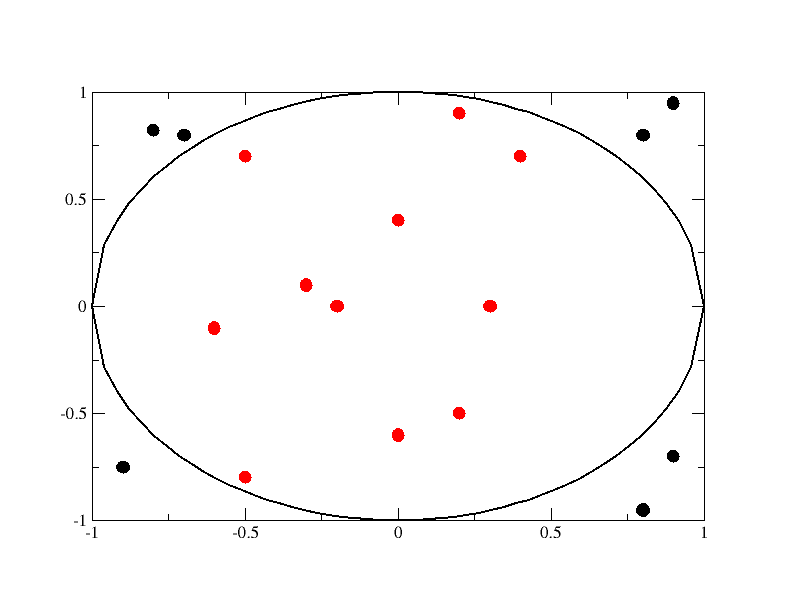
\includegraphics[scale = 0.5]{pi.png}\\
\noindent 3) The ratio of total number of random variable that falls into the circle  to the total number  pair is ratio of the area of the circle to the area of the square\\
\begin{align*}
\frac{ \sum_i^{N} 1_{\pi}}{N} = \pi/4	
\end{align*}
\noindent 4) $\pi$ is equal to $4/N \sum_i^{N} 1_{\pi}$\\
\noindent{\bf b. Proof of (3)}
Based on law of large numbers\\
\begin{align*}
  &\frac{ \sum_i^{N} 1_{\pi}}{N} = E(1_{\pi})\\
= &\int 1_{pi} dP(x,y)\\
= &\int_{-1}^{1} \int_{-1}^{1}  1_{\pi} p(x)p(y) dx dy\\
= &\int_{-1}^{1} \int_{-1}^{1}  1_{\pi} 1/2 1/2 dx dy\\
= & 1/4 \int_{-1}^{1} \int_{-1}^{1}  1_{\pi} dx dy\\
= & 1/4 * \textrm{ area of the circle }\\
= &\pi/4\\	
\end{align*}
$Var(1_{\pi}) < \infty$ since it is a binomial distribution, so $Var(\frac{\sum_i^{N} 1_{\pi}}{N}) =1/N Var(1_{\pi}) = 0$, when N goes to $\infty$
\end{document}